%   % !TEX root = ../../VIII,3_Rahmen-TeX_8-1.tex
%
%
%   Band VIII, 3 N.~??S01.11
%   Signatur/Tex-Datei: LH_37_05_088-089
%   RK-Nr. 57264
%   \ref{dcc_09}
%   Überschrift: De corporum concursus scheda nona
%   Modul: Mechanik / Stoß ( )
%   Datierung: Januar 1678
%   WZ: (Bl. 89) LEd-WZ 803017 = RK-WZ 1264 (insgesamt: eins)
%   SZ:   \groesser   \leibdashv\   \leibdashv\   (insgesamt: drei)
%   Bilddateien (PDF): 
%      LH_37_05_088-089_d1 ((ex: lh37,5,88r))
%      LH_37_05_088-089_d2 ((ex: lh37,5,88v))
%      (insgesamt: zwei)
%   Verzeichniseinträge: vollständig
%   \textls{} statt \textso{} (Ausnahme: Personenverzeichnis)
%
%
\selectlanguage{ngerman}%
\frenchspacing%
%
\begin{ledgroupsized}[r]{120mm}%
\footnotesize%
\pstart%
\noindent%
\textbf{Überlieferung:}%
\pend%
\end{ledgroupsized}%
\begin{ledgroupsized}[r]{114mm}%
\footnotesize%
\pstart%
\parindent -6mm%
\makebox[6mm][l]{\textit{L}}%
Konzept:
LH XXXVII~5, Bl.~88\textendash89.
Ein Bogen 2\textsuperscript{o};
ein Wasserzeichen auf Bl.~89;
unterer Rand von Bl.~89 beschädigt mit Textverlust;
Papiererhaltungsmaßnahmen.
Vier vollbeschriebene Seiten,
die den Text N.~\ref{dcc_08} %??S01\textsubscript{10} 
fortsetzen und vom Text N.~\ref{dcc_10} %??S01\textsubscript{12} 
fortgesetzt werden;
ein Kustos am Ende von Bl.~89~v\textsuperscript{o}\! verweist auf die \textit{Scheda decima}.
\pend%
%
\end{ledgroupsized}%
\begin{ledgroupsized}[r]{114mm}%
\footnotesize%
\pstart%
\parindent -6mm%
\makebox[6mm][l]{\textit{E}}%
\textsc{Fichant} 1994, S.~159\textendash165 (mit kommentierter französischer Übersetzung, S.~317\textendash330).%
\cite{01056}
\pend%
\end{ledgroupsized}%
%
\selectlanguage{latin}%
\frenchspacing%
%
%
\vspace{8mm}
\normalsize%
\count\Bfootins=1000%
\count\Afootins=1200%
\count\Cfootins=1000
\pstart%
\noindent%
%
\lbrack 88~r\textsuperscript{o}\rbrack% \ %%%%    Blatt 88r
\hspace{47mm}
Scheda nona%
\protect\index{Sachverzeichnis}{scheda}%
\hspace{38mm}
Januar.\ 1678%
\pend%
\vspace{0.5em}%
%
\pstart%
\noindent%
Tentandum%
\edlabel{LH_37_05_088rv_cntrmgrvtts-1}
an demonstrare liceat regulam de via centri gravitatis%
\protect\index{Sachverzeichnis}{regula de via centri gravitatis}
in corporum motibus concursibusque servanda,%
\protect\index{Sachverzeichnis}{concursus corporum}%
\protect\index{Sachverzeichnis}{via centri gravitatis servanda}
quod si effecerimus
rem maximam in phoronomica egerimus.%
\protect\index{Sachverzeichnis}{phoronomica}
\pend%
%
\pstart%
\edtext{Torricellius%
\protect\index{Namensregister}{\textso{Torricelli} (Torricellius), Evangelista 1608\textendash1647}
demonstravit in machina quavis%
\protect\index{Sachverzeichnis}{machina}
continue centrum gravitatis deorsum tendere.%
\protect\index{Sachverzeichnis}{centrum gravitatis machinae}%
\protect\index{Sachverzeichnis}{centrum gravitatis deorsum tendens}%
\edlabel{LH_37_05_088-089_lxtd-1}%
}{%
\lemma{Torricellius \lbrack...\rbrack\ tendere}\Cfootnote{%
Vgl. \textsc{E.~Torricelli}, \textit{De motu gravium}, lib.~I
(\cite{00304}\textit{Opera geometrica}, Florenz 1644, S.~99;
\cite{00108}\textit{TO}~II, S.~105).%
}}
%
\edtext{}{% B-Footnote: "tendere. Idem"
{\xxref{LH_37_05_088-089_lxtd-1}{LH_37_05_088-089_lxtd-2}}%
{\lemma{tendere.}%
\Bfootnote{%
\textit{(1)}~Hinc etiam demonstratur
\textit{(2)}~Idem Pascalius \lbrack...\rbrack\ demonstratum asserunt,%
~\textit{L}}}}%
%
\edtext{Idem Pascalius%
\protect\index{Namensregister}{\textso{Pascal} (Pascalius), Blaise 1623\textendash1662}
aliique a se demonstratum asserunt,%
\edlabel{LH_37_05_088-089_lxtd-2}%
}{%
\lemma{Idem \lbrack...\rbrack\ asserunt}%
\Cfootnote{%
Wohl Anspielung auf
\textsc{B.~Pascal}, \textit{Traité de l'équilibre des liqueurs}, chap.~2
(Paris 1663, S.~10f.;\cite{00081} \textit{PO} III, S.~166f.\cite{00234});
Pascal beweist den Satz allerdings nicht, sondern nimmt ihn als Grundsatz an.
Leibniz hat aus diesem Kapitel 1672 einen Auszug verfasst; siehe \textit{LSB} VIII,~1 N.~38, S.~289.14\textendash17.\edlabel{01038}}}
%
sed non difficilis est
%
\edtext{}{%
{\xxref{LH_37_05_088r_xvgjn-1}{LH_37_05_088r_xvgjn-2}}%
{\lemma{demonstratio \lbrack...\rbrack\ perpetuus}\Cfootnote{%
Ähnlicher Ansatz bereits in
N.~\ref{RK60282};
N.~\ref{RK60278};
N.~\ref{RK57266-1}, S.~\refpassage{LH_37_05_162r_Gedankenexperiment-1}{LH_37_05_162r_Gedankenexperiment-2}.%
}}}%
\edlabel{LH_37_05_088r_xvgjn-1}%
demonstratio,%
\protect\index{Sachverzeichnis}{demonstratio}
vel ex eo
quod alioqui motus%
\protect\index{Sachverzeichnis}{motus perpetuus artificialis}
%
\edtext{perpetuus.%
\edlabel{LH_37_05_088r_xvgjn-2}
Limitandum est tamen%
\lbrack:\rbrack\
si corpus non novo impulsu feratur,%
\protect\index{Sachverzeichnis}{impulsus novus}
sed quaesita semel celeritate.%
\protect\index{Sachverzeichnis}{celeritas quaesita}%
}{%
\lemma{per-}\Bfootnote{% ! ! ! ! ACHTUNG GETRIXT ! ! ! !
\hspace{-0,5mm}petuus.
\textit{(1)}~Hinc jam porro colligo: si duo corpora quae non ferantur accelerata
\textit{(a)}~celeritate
\textit{(b)}~vi, sed ea quam semel habent
\textit{(2)}~Limitandum est % tamen si corpus non novo impulsu feratur, sed quaesita
\lbrack...\rbrack\ semel celeritate.%
~\textit{L}}}
%
Itaque casus accelerationum hinc removendus.%
\protect\index{Sachverzeichnis}{acceleratio}
Sed tamen et hunc licebit salvare,
si ope accelerationum%
\protect\index{Sachverzeichnis}{acceleratio}
ponas caeteris
%
\edtext{paribus%
\lbrack;\rbrack\
et quando ita%
\lbrack,\rbrack\
licet centrum gravitatis}{%
\lemma{paribus}\Bfootnote{%
\textit{(1)}~centrum gravit
\textit{(2)}~et quando % ita licet 
\lbrack...\rbrack\ centrum gravitatis%
~\textit{L}}}
%
aequaliter ascendere ac descendit.%
\protect\index{Sachverzeichnis}{centrum gravitatis ascendens}%
\protect\index{Sachverzeichnis}{centrum gravitatis descendens}
\pend%
%
\pstart%
In%
\protect\index{Sachverzeichnis}{liquidum}
%
\edtext{liquido sint}{%
\lemma{liquido}\Bfootnote{%
\textit{(1)}~descendant
\textit{(2)}~sint%
~\textit{L}}}
%
duo corpora,
unum gravitate specifica descendens,%
\protect\index{Sachverzeichnis}{corpus gravitate specifica descendens}%
\protect\index{Sachverzeichnis}{gravitas specifica}
alterum levitate specifica ascendens%
\protect\index{Sachverzeichnis}{corpus levitate specifica ascendens}%
\protect\index{Sachverzeichnis}{levitas specifica}%
\lbrack,\rbrack\
et quidem motu uniformi%
\protect\index{Sachverzeichnis}{motus uniformis}%
\lbrack;\rbrack\
quod fit
cum ad eam accelerationem pervenere,%
\protect\index{Sachverzeichnis}{acceleratio}
ut ferri possint a liquido ipso%
\protect\index{Sachverzeichnis}{liquidum}
tanta celeritate moto.%
\protect\index{Sachverzeichnis}{celeritas liquidi}
Patet ante ictum%
\protect\index{Sachverzeichnis}{ictus corporum in liquido}
eorum centrum gravitatis descendere uniformiter,%
\protect\index{Sachverzeichnis}{centrum gravitatis descendens}
ponamus post ictum%
\protect\index{Sachverzeichnis}{ictus corporum in liquido}
id rursus ascendere,%
\protect\index{Sachverzeichnis}{centrum gravitatis ascendens}
ergo si satis altus est liquor%
\protect\index{Sachverzeichnis}{liquor}
statim obtinebimus motum perpetuum artificialem%
\protect\index{Sachverzeichnis}{motus perpetuus artificialis}%
\lbrack;\rbrack\
igitur pro certo habendum est,
si duo corpora in liquore%
\protect\index{Sachverzeichnis}{liquor}
vel recta vel plano inclinato%
\protect\index{Sachverzeichnis}{planum inclinatum}
uniformi celeritate%
\protect\index{Sachverzeichnis}{celeritas uniformis}
hoc modo concurrant,%
\protect\index{Sachverzeichnis}{corpora in liquore concurrentia}
centrum gravitatis eorum continuabit motum%
\protect\index{Sachverzeichnis}{motus centri gravitatis}
in eandem semper
%
\edtext{partem.%
\protect\index{Sachverzeichnis}{directio centri gravitatis}
Si autem}{%
\lemma{partem.}\Bfootnote{%
\textit{(1)}~Quod si
\textit{(2)}~Si autem%
~\textit{L}}}
%
reverteretur in contrariam,
statim ostendam haberi motum perpetuum%
\protect\index{Sachverzeichnis}{motus perpetuus artificialis}%
\lbrack:\rbrack\
nam si resurgit,%
\protect\index{Sachverzeichnis}{centrum gravitatis resurgens}
ponamus
%
\edtext{tandem%
\lbrack,\rbrack\
ubi altius assurexit}{%
\lemma{tandem}\Bfootnote{%
\textit{(1)}~connecti corpora per lineam
\textit{(2)}~ubi latus est
\textit{(3)}~ubi altius assurexit%
~\textit{L}}}
%
quam unde venit,
corpora per lineam rigidam%
\protect\index{Sachverzeichnis}{linea rigida}
connecti;%
\protect\index{Sachverzeichnis}{corpora per linea rigida connexa}
tunc iterum descendet%
\protect\index{Sachverzeichnis}{centrum gravitatis descendens}
ut ante concursum\lbrack;\rbrack\ %,
unde ponamus lineam rigidam%
\protect\index{Sachverzeichnis}{linea rigida}
iterum dissolvi
ubi libuerit,
iterum ascendet,%
\protect\index{Sachverzeichnis}{centrum gravitatis ascendens}
et ita habebitur haud dubie motus perpetuus artificialis.%
\protect\index{Sachverzeichnis}{motus perpetuus artificialis}
\pend%
%
\pstart%
Quaeritur jam
an post ictum%
\protect\index{Sachverzeichnis}{ictus}
%
\edtext{eadem celeritate}{%
\lemma{eadem}\Bfootnote{%
\textit{(1)}~linea
\textit{(2)}~celeritate%
~\textit{L}}}
%
pergat centrum gravitatis,%
\protect\index{Sachverzeichnis}{celeritas centri gravitatis}%
\protect\index{Sachverzeichnis}{centrum gravitatis pergens post ictum}
qua
%
\edtext{ante.
Fingamus motum esse}{%
\lemma{ante}\Bfootnote{%
\textit{(1)}~, et durante motu corpora linea rigida connecti, utique
\textit{(2)}~. Fingamus motum esse%
~\textit{L}}}
%
in tubo inclinato,%
\protect\index{Sachverzeichnis}{tubus inclinatus}%
\protect\index{Sachverzeichnis}{motus in tubo inclinato}
tubum autem ipsum non ponderare in liquido%
\protect\index{Sachverzeichnis}{liquidum}%
\protect\index{Sachverzeichnis}{tubus non ponderans in liquido}
%
\edtext{ob materiam.%
\protect\index{Sachverzeichnis}{materia}}{%
\lemma{\textit{Am Rand,
auf} ob materiam \textit{bezogen:}}\Afootnote{%
tubus liquore plenus forte clausus%
\protect\index{Sachverzeichnis}{tubus liquore plenus}%
\protect\index{Sachverzeichnis}{liquor}%
}}
%
Caeterum centrum%
\protect\index{Sachverzeichnis}{centrum suspensionis tubi}
ex quo tubus inclinate sit suspensus%
\protect\index{Sachverzeichnis}{tubus inclinate suspensus}
%
\edtext{incedere et}{%
\lemma{incedere}\Bfootnote{%
\hspace{-0,5mm}et
\textit{erg.~L}}}
%
moveri
%
\edtext{sub tubo}{%
\lemma{sub}\Bfootnote{%
\hspace{-0,5mm}tubo
\textit{erg.~L}}}
%
eodem prorsus modo,
ut centrum gravitatis corporum%
\protect\index{Sachverzeichnis}{corpus in tubo motum}%
\protect\index{Sachverzeichnis}{tubus inclinatus}%
\protect\index{Sachverzeichnis}{tubus inclinate suspensus}
in tubo motorum%
\protect\index{Sachverzeichnis}{centrum gravitatis corporum in tubo}
ante concursum,%
\protect\index{Sachverzeichnis}{concursus corporum in tubo}
eodemque
%
\edtext{modo etiam post concursum%
\protect\index{Sachverzeichnis}{concursus corporum in tubo}
hoc centrum suspensionis tubi pergere;%
\protect\index{Sachverzeichnis}{centrum suspensionis tubi}%
}{%
\lemma{modo}\Bfootnote{%
\textit{(1)}~pergere,
\textit{(2)}~etiam post concursum hoc
\textit{(a)}~eo
\textit{(b)}~hoc centrum suspensionis tubi pergere;%
~\textit{L}}}
%
ipsum vero
%
\edtext{centrum gravitatis corporum%
\protect\index{Sachverzeichnis}{centrum gravitatis corporum in tubo}%
}{%
\lemma{gravitatis}\Bfootnote{%
\textit{(1)}~tuborum
\textit{(2)}~corporum%
~\textit{L}}}
%
ponamus aliter moveri post ictum,%
\protect\index{Sachverzeichnis}{ictus corporum in tubo}
utique statim tubus circumagetur%
\protect\index{Sachverzeichnis}{tubus circumactus}
%
\edtext{nonnihil}{%
\lemma{nonnihil}\Bfootnote{%
\textit{erg.~L}}}
%
ob eorum pondera.
Ponamus tamen illam circumactionem impediri,%
\protect\index{Sachverzeichnis}{circumactio tubi}
donec eousque diversitas
inter centrum suspensionis tubi%
\protect\index{Sachverzeichnis}{centrum suspensionis tubi}
et centrum gravitatis corporum pervenerit,%
\protect\index{Sachverzeichnis}{centrum gravitatis corporum in tubo}
ut permissa circumactione%
\protect\index{Sachverzeichnis}{circumatio tubi}
centrum gravitatis iterum deprimatur vel ascendat,%
\protect\index{Sachverzeichnis}{centrum gravitatis depressum}%
\protect\index{Sachverzeichnis}{centrum gravitatis ascendens}
donec coincidant centrum suspensionis%
\protect\index{Sachverzeichnis}{centrum suspensionis tubi}
et
%
\edtext{levitatis.%
\protect\index{Sachverzeichnis}{centrum levitatis}%
}{%
\lemma{levitatis}\Cfootnote{%
Gemeint ist wohl doch das \textit{centrum gravitatis}.%
}}
%
Quo facto,
hinc aliquam vim obtinuimus;%
\protect\index{Sachverzeichnis}{vis obtenta}
imo poterimus efficere reciprocationes etc.%
\protect\index{Sachverzeichnis}{reciprocatio}
Sed hoc distinctius explicandum.
\pend%
%
%
%  \newpage% 
  \vspace{1.5em}%	% Diagramm Fig.~1
  \centerline{\includegraphics[width=0.58\textwidth]{gesamttex/edit_VIII,3/images/LH_37_05_088-089_d1.pdf}}%
  \vspace{0.5em}
  \centerline{\lbrack\textit{Fig.~1}\rbrack}%
  \label{LH_37_05_088r_Fig.1}%
%  \vspace{1.5em}%
  \newpage%
%
%
\pstart%
%
\edtext{Sit libra,%
\protect\index{Sachverzeichnis}{libra}%
}{%
\lemma{Sit libra}\Cfootnote{%
Siehe das Diagramm \lbrack\textit{Fig.~1}\rbrack\
auf S.~\pageref{LH_37_05_088r_Fig.1}.}}
%
cujus brachia%
\protect\index{Sachverzeichnis}{brachium librae}
sustineant plana horizontalia,%
\protect\index{Sachverzeichnis}{planum horizontale}
in quibus utrinque similiter
%
\edtext{corpora versus se invicem currant,%
\protect\index{Sachverzeichnis}{corpora versus se invicem currentia}%
}{%
\lemma{corpora}\Bfootnote{%
\textit{(1)}~concurrant
\textit{(2)}~versus se invicem currant,%
~\textit{L}}}
%
sit \textit{b} aequ. \textit{B},
et \textit{a} aequ. \textit{A}.
%
\edtext{Itaque cum semel sit}{%
\lemma{Itaque}\Bfootnote{%
\textit{(1)}~si semel
\textit{(2)}~cum semel%
~\textit{L}}}
%
libra in aequilibrio;%
\protect\index{Sachverzeichnis}{aequilibrium librae}%
\protect\index{Sachverzeichnis}{libra}
durante motu manebit in aequilibrio%
\protect\index{Sachverzeichnis}{aequilibrium librae}
quia utrobique centrum gravitatis corporum%
\protect\index{Sachverzeichnis}{centrum gravitatis corporum concurrentium}
eodem modo recedet a centro librae%
\protect\index{Sachverzeichnis}{centrum librae}
vel ad ipsum accedet.
Ponamus jam duo corpora in uno latere concurrere,%
\protect\index{Sachverzeichnis}{corpora concurrentia}
in altero se nonnihil evitare,%
\protect\index{Sachverzeichnis}{corpora se evitantia}
et in his manere viam centri,%
\protect\index{Sachverzeichnis}{via centri gravitatis manens}
in alteris vero mutari,%
\protect\index{Sachverzeichnis}{via centri gravitatis mutans}
necessario brachium librae%
\protect\index{Sachverzeichnis}{brachium librae}
inclinabitur ab alterutra parte;
ponamus autem corpora post concursum%
\protect\index{Sachverzeichnis}{concursus corporum}
reflecti%
\protect\index{Sachverzeichnis}{corpus reflexum}%
\protect\index{Sachverzeichnis}{reflexio corporum concurrentium}
iterum ab extremis
%
\edtext{lancis%
\protect\index{Sachverzeichnis}{lanx librae}%
\lbrack,\rbrack\
quaeque suae,}{%
\lemma{lancis}\Bfootnote{%
\textit{(1)}~unumquodque su
\textit{(2)}~quaeque suae,%
~\textit{L}}}
%
et alternis jam evitare
%
\edtext{se%
\protect\index{Sachverzeichnis}{corpora se evitantia}
quae antea}{%
\lemma{se}\Bfootnote{%
\textit{(1)}~priora
\textit{(2)}~quae antea%
~\textit{L}}}
%
concurrerant,
concurrere altera%
\protect\index{Sachverzeichnis}{corpora concurrentia}%
\lbrack:\rbrack\
iterum inclinabitur rursus
%
\edtext{\lbrack brachium\rbrack%
\protect\index{Sachverzeichnis}{brachium librae}%
}{%
\lemma{tubus}\Bfootnote{%
\textit{L~ändert Hrsg. nach~E, S.~160}\cite{01056}%
\protect\index{Sachverzeichnis}{tubus}%
}}
%
in aliam partem,
et
%
\edtext{ita habebitur}{%
\lemma{ita}\Bfootnote{\hspace{-0,5mm}%
\textbar~manifeste \textit{gestr.}~%
\textbar\ habebitur%
~\textit{L}}}
%
motus perpetuus.%
\protect\index{Sachverzeichnis}{motus perpetuus artificialis}
Sane certum est
hoc modo augeri
%
\edtext{\lbrack aliquantum\rbrack}{%
\lemma{alioqui}\Bfootnote{%
\textit{L~ändert Hrsg.}}}
%
vim,%
\protect\index{Sachverzeichnis}{vis aucta}
quia eo ipso,
dum mutatio%
\protect\index{Sachverzeichnis}{mutatio librae}
%
\edtext{fit,
seu ascensus%
\protect\index{Sachverzeichnis}{ascensus librae}
et descensus%
\protect\index{Sachverzeichnis}{descensus librae}
aliquis fit,
vim aliquam lucramur,%
\protect\index{Sachverzeichnis}{vis lucrata}%
\protect\index{Sachverzeichnis}{lucratio virium}%
}{%
\lemma{fit}\Bfootnote{%
\textit{(1)}~augetur vis
\textit{(2)}~seu ascensus % et descensus aliquis fit, vim 
\lbrack...\rbrack\ aliquam lucramur,%
~\textit{L}}}
%
nulla alia vi perdita.%
\protect\index{Sachverzeichnis}{vis perdita}
\pend%
%
\pstart%
Faciendum
ut semper sit \textit{AB} horizonti parallela,%
\protect\index{Sachverzeichnis}{horizon}
sive ascendat sive descendat libra%
\protect\index{Sachverzeichnis}{libra ascendens}%
\protect\index{Sachverzeichnis}{libra descendens}
et ubicunque sit centrum gravitatis corporum%
\protect\index{Sachverzeichnis}{centrum gravitatis corporum in libra}
in qualibet lance.%
\protect\index{Sachverzeichnis}{lanx librae}
Possunt et adhiberi pendula vibrantia%
\protect\index{Sachverzeichnis}{pendulum vibrans}
in librae lance%
\protect\index{Sachverzeichnis}{lanx librae}
separatim suspensa.%
\protect\index{Sachverzeichnis}{pendulum in libra suspensum}
%
\lbrack88~v\textsuperscript{o}\rbrack\ %%%%    Blatt 88v
%
%\pend%
%%
%\pstart%
Ut semper plana illa horizonti parallela maneant,%
\protect\index{Sachverzeichnis}{planum horizonti parallelum}
sic efficiemus.
Sit linea \textit{AB} immobilis,
%
\edtext{vel sufficit puncta \textit{A}, \textit{B} esse immobilia.}{%
\lemma{vel}\Bfootnote{%
\hspace{-0,5mm}sufficit % puncta \textit{A}, \textit{B} 
\lbrack...\rbrack\ esse immobilia
\textit{erg.~L}}}
%
Patet
circa ipsam velut libram%
\protect\index{Sachverzeichnis}{libra}
moveri \textit{EF} et \textit{CD},
nam ascendente \textit{CD} descendit \textit{EF} et contra.
Rectae autem \textit{EF}, \textit{CD}
semper manent inter se
et horizontali immobili \textit{AB} parallelae.
\pend%
%
%
%  \newpage% 
  \vspace{1.5em}%	% Diagramm Fig.~2
  \centerline{\hspace{10mm}\includegraphics[width=0.42\textwidth]{gesamttex/edit_VIII,3/images/LH_37_05_088-089_d2.pdf}}%
  \vspace{0.5em}
  \centerline{\hspace{5mm}\lbrack\textit{Fig.~2}\rbrack}%
%  \label{LH_37_05_088v_Fig.2}%
%  \vspace{1.5em}%
  \newpage%
%
%
\pstart%
%\begin{wrapfigure}{l}{0.4\textwidth}
%\includegraphics[width=0.38\textwidth]{gesamttex/edit_VIII,3/images/lh37,5,88v.pdf}
%\noindent \centering [\textit{Fig.~2}]
%\end{wrapfigure}
Si jam
%
\edtext{corpora \textit{G},\,\textit{H} concurrant%
\protect\index{Sachverzeichnis}{corpora concurrentia}
in recta \textit{CD},
et corpora \textit{L},\,\textit{M} in recta \textit{EF},%
}{%
\lemma{corpora}\Bfootnote{%
\hspace{-0,5mm}\textit{G}~\textit{H}
\textit{(1)}~et \textit{L}~\textit{M}
\textit{(2)}~concurrant in recta
\textit{(a)}~\textit{EF}, et
\textit{(b)}~\textit{CD},%
~\textit{L}}}
%
ita ut sit \textit{L} simile et aequale ipsi \textit{H},
et \textit{M} simile et aequale ipsi \textit{G},
sitque \textit{CG} aequ. \textit{FM},
et \textit{DH} aequ. \textit{EL},
atque ita concurrant eodem modo
in uno pariter atque altero plano,
patet ante
%
\edtext{concursum%
\protect\index{Sachverzeichnis}{concursus corporum}
centrum gravitatis eodem modo supra infraque moveri,%
\protect\index{Sachverzeichnis}{centrum gravitatis eodem modo movens}%
\protect\index{Sachverzeichnis}{motus centri gravitatis}%
}{%
\lemma{concursum}\Bfootnote{%
\textit{(1)}~manere semper idem
\textit{(2)}~centrum gravitatis % eodem modo supra 
\lbrack...\rbrack\ infraque moveri,%
~\textit{L}}}
%
ita ut semper libra%
\protect\index{Sachverzeichnis}{libra in aequilibrio}
maneat in aequilibrio%
\protect\index{Sachverzeichnis}{aequilibrium librae}
si semel in eo fuit.
Quod si vero idem non contingit post concursum%
\protect\index{Sachverzeichnis}{concursus corporum}
%
\edtext{supponendo inferiora concurrere,%
\protect\index{Sachverzeichnis}{corpora concurrentia}
superiora se evitare%
\protect\index{Sachverzeichnis}{corpora se evitantia}
seu unum prope alterum decurrere%
\lbrack,\rbrack%
}{%
\lemma{supponendo}\Bfootnote{%
\hspace{-0,5mm}inferiora % concurrere superiora se evitare seu unum prope 
\lbrack...\rbrack\ alterum decurrere
\textit{erg.~L}}}
%
necesse est cessante aequilibrio%
\protect\index{Sachverzeichnis}{aequilibrium librae}
et centro gravitatis corporum%
\protect\index{Sachverzeichnis}{centrum gravitatis corporum in libra}
in una lance \textit{CD} aliter posito
quam centro gravitatis corporum in altera lance%
\protect\index{Sachverzeichnis}{lanx librae}
%
\edtext{\textit{EF},
libram mutari%
\protect\index{Sachverzeichnis}{libra mutans}%
\protect\index{Sachverzeichnis}{mutatio librae}
et alterutram lancem \textit{CD} vel \textit{EF}%
\protect\index{Sachverzeichnis}{lanx librae}%
}{%
\lemma{\textit{EF},}\Bfootnote{\hspace{-0,5mm}%
\textbar~tamen \textit{gestr.}~%
\textbar\ libram mutari et
\textit{(1)}~alterutrum \textit{CD}
\textit{(2)}~alterutram lancem \textit{CD} vel \textit{EF}%
~\textit{L}}}
%
cum suis corporibus ascendere vel descendere\lbrack,\rbrack %;%
\protect\index{Sachverzeichnis}{ascensus librae}%
\protect\index{Sachverzeichnis}{descensus librae}
et quidem determinata quadam vi,%
\protect\index{Sachverzeichnis}{vis librae}
quae etiam aliquod extra libram movere possit;%
\protect\index{Sachverzeichnis}{vis movens}
ita
%
\edtext{jam aliquem motum%
\protect\index{Sachverzeichnis}{motus lucratus}%
\protect\index{Sachverzeichnis}{lucratio motus}%
}{%
\lemma{jam}\Bfootnote{%
\textit{(1)}~motum
\textit{(2)}~aliquem motum%
~\textit{L}}}
%
vel vim aliquam%
\protect\index{Sachverzeichnis}{vis lucrata}%
\protect\index{Sachverzeichnis}{lucratio virium}
lucrati erimus sine causa%
\protect\index{Sachverzeichnis}{causa lucrationis}%
\protect\index{Sachverzeichnis}{lucratio sine causa}%
\lbrack,\rbrack\
Eam scilicet quae lancem facit inclinari,
cum tamen interim vis%
\protect\index{Sachverzeichnis}{vis machinae}
%
\edtext{quae jam antea erat in machina,%
\protect\index{Sachverzeichnis}{machina}%
}{%
\lemma{quae}\Bfootnote{%
\textit{(1)}~esset in
\textit{(2)}~jam antea erat in machina,%
~\textit{L}}}
%
id est quae corpora discurrere facit,%
\protect\index{Sachverzeichnis}{vis corpora discurrere faciens}%
\protect\index{Sachverzeichnis}{corpora discurrentia}
ex hypothesi eadem manserit.%
\protect\index{Sachverzeichnis}{hypothesis}
Quod est absurdum.%
\protect\index{Sachverzeichnis}{absurdum}
Necesse est ergo
manere semper eandem viam centri gravitatis%
\protect\index{Sachverzeichnis}{via centri gravitatis eadem manens}
corporum ante et post concursum.%
\protect\index{Sachverzeichnis}{concursus corporum}
\pend%
%
\pstart%
Si secus contingeret,
hac machina%
\protect\index{Sachverzeichnis}{machina motum perpetuum habens}
haberetur motus perpetuus artificialis%
\protect\index{Sachverzeichnis}{motus perpetuus artificialis}
posita corporum duritie satis perfecta et durabili.%
\protect\index{Sachverzeichnis}{durities perfecta}%
\protect\index{Sachverzeichnis}{durities durabilis}
%
\edtext{Nam ponamus corpora}{%
\lemma{Nam}\Bfootnote{%
\textit{(1)}~corporibus
\textit{(2)}~ponamus corpora%
~\textit{L}}}
%
infra concurrentia iterum%
\protect\index{Sachverzeichnis}{corpora concurrentia}
servato toto motu%
\protect\index{Sachverzeichnis}{motus servatus}
%
\edtext{reflecti%
\protect\index{Sachverzeichnis}{corpus reflexum}
et versus extrema}{%
\lemma{reflecti}\Bfootnote{%
\hspace{-0,5mm}et
\textit{(1)}~recurrere versus
\textit{(2)}~versus extrema%
~\textit{L}}}
%
lancis recurrere,%
\protect\index{Sachverzeichnis}{lanx librae}
et ab illis quippe immobilibus
(\protect\vphantom)%
secundum hanc lineam motus%
\protect\vphantom()
et durissimis reflecti pilas%
\protect\index{Sachverzeichnis}{pila reflexa}
etiam integro servato motu,%
\protect\index{Sachverzeichnis}{motus servatus}
necessario denuo concurrent%
\protect\index{Sachverzeichnis}{concursus corporum}
et denuo reflectentur;%
\protect\index{Sachverzeichnis}{reflexio corporum concurrentium}
idque sine fine,
qui est motus perpetuus naturalis.%
\protect\index{Sachverzeichnis}{motus perpetuus naturalis}
Idem contingeret in superiori lance \textit{EF}%
\protect\index{Sachverzeichnis}{lanx librae}
etiamsi ibi se evitent,
nihilominus ab extremis reflectentur
et se porro evitabunt.%
\protect\index{Sachverzeichnis}{corpora se evitantia}
Porro cum durantibus his reflexionibus%
\protect\index{Sachverzeichnis}{reflexio corporum concurrentium}
et discursibus%
\protect\index{Sachverzeichnis}{discursus corporum}
multis
%
\edtext{modis variatum}{%
\lemma{modis}\Bfootnote{%
\textit{(1)}~variata
\textit{(2)}~variatum%
~\textit{L}}}
%
iri centra gravitatis lancium,%
\protect\index{Sachverzeichnis}{centrum gravitatis lancis librae}%
\protect\index{Sachverzeichnis}{variatio centri gravitatis}
et nunc unum nunc alterum
propius centro motus%
\protect\index{Sachverzeichnis}{centrum motus librae}
futurum esse
pateat,
manifestum est etiam
libram in perpetua fore vacillatione%
\protect\index{Sachverzeichnis}{libra vacillans}%
\protect\index{Sachverzeichnis}{vacillatio librae perpetua}
satis forti ad aliam rotam extra libram circumagendam,%
\protect\index{Sachverzeichnis}{rota circumagenda}
ipsa interim machina in libra inclusa%
\protect\index{Sachverzeichnis}{machina in libra inclusa}%
\protect\index{Sachverzeichnis}{machina vim retinens}
totam vim suam retinente.%
\protect\index{Sachverzeichnis}{vis machinae}%
\protect\index{Sachverzeichnis}{vis retenta}
\pend%
%
\pstart%
\edtext{%
Hinc%
\edlabel{LH_37_05_088v_SchwerpunktBeweis-1}
etiam patet,
licet corpora sint mollia utcunque,%
\protect\index{Sachverzeichnis}{corpus molle}
tamen
si progrediantur%
\protect\index{Sachverzeichnis}{corpus progrediens}
eorum centrum gravitatis eodem modo progredi debere.%
\protect\index{Sachverzeichnis}{progressus centri gravitatis}%
\protect\index{Sachverzeichnis}{centrum gravitatis eodem modo progrediens}
Idemque non solum
%
\edtext{in corporibus sphaericis,%
\protect\index{Sachverzeichnis}{corpus sphaericum}
sed et quibuscunque locum}{%
\lemma{corporibus}\Bfootnote{%
\textit{(1)}~duris, sed et mollibus
\textit{(2)}~sphaericis, sed et quibuscunque%
~\textit{L}}}
%
habere;
nec numerum etiam corporum%
\protect\index{Sachverzeichnis}{numerus corporum concurrentium}
quicquam ad rem pertinere.}{\lemma{Hinc \lbrack...\rbrack\ pertinere}\Cfootnote{%
Vgl. die Schlussbemerkung in \textsc{C.~Huygens},
\cite{01067}\glqq A summary account of the laws of motion\grqq\
(\textit{PT} IV, 1669, S.~928;
\cite{00113}\textit{HO} VI, S.~433).%
}}
%
Hinc etiam si plura corpora%
\protect\index{Sachverzeichnis}{corpora concurrentia}
%
\edtext{concurrant
colligere}{%
\lemma{concurrant}\Bfootnote{\hspace{-0,5mm}%
\textbar~hinc \textit{streicht Hrsg.}~%
\textbar\ colligere%
~\textit{L}}}
%
aliquid licebit,
et quia tunc pluribus modis salvari possunt%
\lbrack,\rbrack\
haec duae:
conservatio directionis,%
\protect\index{Sachverzeichnis}{conservatio directionis centri gravitatis}
et conservatio virium.%
\protect\index{Sachverzeichnis}{conservatio virium corporum concurrentium}%
\edlabel{LH_37_05_088v_SchwerpunktBeweis-2}%
\edlabel{LH_37_05_088rv_cntrmgrvtts-2}
%
\lbrack89~r\textsuperscript{o}\rbrack\ %%%%    Blatt 89r
%
\pend%
%
\pstart%
Superest ut percussionem%
\protect\index{Sachverzeichnis}{percussio eadem}
%
\edtext{examinemus.
Et primum quaestio illa tractanda,%
\protect\index{Sachverzeichnis}{quaestio de percussione}
an eadem sit percussio,%
\protect\index{Sachverzeichnis}{percussio eadem}%
}{%
\lemma{examinemus}\Bfootnote{%
\textit{(1)}~an eadem \textlangle sit\textrangle\
\textit{(2)}~. Et primum % quaestio illa tractanda, an eadem 
\lbrack...\rbrack\ sit percussio,%
~\textit{L}}}
%
quandocunque corpora concurrunt%
\protect\index{Sachverzeichnis}{corpora pari celeritate appropinquationis concurrentia}
pari celeritate appropinquationis,%
\protect\index{Sachverzeichnis}{celeritas appropinquationis}
%
\edtext{etiamsi non eadem sit}{%
\lemma{etiamsi}\Bfootnote{%
\textit{(1)}~eadem sit
\textit{(2)}~non eadem sit%
~\textit{L}}}
%
eorum celeritas.%
\protect\index{Sachverzeichnis}{celeritas corporum concurrentium}
Sint
%
\edtext{corpora \textit{a}, \textit{b}.
Ponatur distantia \textit{d}%
\protect\index{Sachverzeichnis}{distantia corporum concurrentium}
et solum \textit{a} moveri celeritate \textit{d},%
\protect\index{Sachverzeichnis}{celeritas corporum concurrentium}
erit vis corporum $ad^2.$%
\protect\index{Sachverzeichnis}{vis corporum concurrentium}%
}{%
\lemma{corpora}\Bfootnote{%
\hspace{-0,5mm}\textit{a},~\textit{b}
\textit{(1)}~quorum celeritates $\omega$~\textit{i}. Ponatur primum \textit{i} aequ. 0 et
\textit{(a)}~sit
\textit{(b)}~erit tota
\textit{(2)}~. Ponatur distantia \lbrack...\rbrack\ corporum $ad^2.$%
~\textit{L}}}
%
Distantia autem corporum%
\protect\index{Sachverzeichnis}{distantia corporum concurrentium}
ex qua concurrunt
erit \textit{d}.
Ponamus jam eadem concurrere ex eadem distantia,
%
\edtext{sed celeritate}{%
\lemma{sed}\Bfootnote{%
\textit{(1)}~motu virium
\textit{(2)}~celeritate%
~\textit{L}}}
%
ponderibus
\edlabel{LH_37_05_089r_cxgo-1}%
reciproca,%
\protect\index{Sachverzeichnis}{celeritas concursus ponderibus reciproca}%
%
\edtext{}{%
{\xxref{LH_37_05_089r_cxgo-1}{LH_37_05_089r_cxgo-2}}%
{\lemma{reciproca,}\Bfootnote{%
\textit{(1)}~nempe $ae^2$
\textit{(2)}~ipsius \textit{a} \lbrack...\rbrack\ et $ae^2$%
~\textit{L}}}}%
%
\pend%
\vspace{0.5em}
%
\pstart%
\noindent%
\lbrack \textit{Nachfolgend klein gedruckter Text in L gestrichen:}\rbrack%
\pend%
\vspace{0.5em}
%
\footnotesize%
\pstart%
\noindent%
%
ipsius \textit{a} celeritas sit \textit{e},
et ipsius \textit{b} celeritas \textit{i},
et
%
\edtext{$ae^2$%
\edlabel{LH_37_05_089r_cxgo-2}
aequ. $bi^2,$}{%
\lemma{$ae^2$ aequ. $bi^2$}\Cfootnote{%
Dies widerspricht der soeben getroffenen Setzung $e : i = b : a.$%
}}
%
et $e+i$ aequ. \textit{d}.
Quaeritur an 
%
\edtext{$ae^2+bi^2$ possit esse majus quam $ad^2.$
Patet}{%
\lemma{$ae^2+bi^2$}\Bfootnote{%
\textit{(1)}~sit majus vel
\textit{(2)}~possit esse majus quam $ad^2$
\textbar~vel \textit{erg.~L, streicht Hrsg.}~%
\textbar~. Patet
~\textit{L}}}
%
$ad^2$ esse aequ. $ae^2+ai^2+2aei.$%
\rule[0mm]{0mm}{4mm}
Ergo sublata $ae^2$ utrinque,
quaeritur
an possit $bi^2$ esse majus quam $ai^2+2aei$
seu an \textit{bi} possit esse majus quam $ai+2ae,$
%
\edtext{id est
an $\displaystyle \frac{b}{a}$}{%
\lemma{id est}\Bfootnote{%
\textit{(1)}~an \textit{i}
\textit{(2)}~an $\displaystyle \frac{b}{a}$%
~\textit{L}}}
%
possit esse majus quam
$\displaystyle \frac{i+2e}{i}.$
Quod utique alioqui fieri posse
constat
%
\edtext{ex prioribus,}{%
\lemma{ex prioribus}\Cfootnote{%
Vgl. N.~\ref{dcc_08}, %??S01\textsubscript{10},
S.~\refpassage{LH_37_05_087v_regula_kdkq-1}{LH_37_05_087v_regula_kdkq-2};
\refpassage{LH_37_05_087v_regula_afnj-1}{LH_37_05_087v_regula_afnj-2}.%
}}
%
imo semper fieri
quando corpus \textit{b} est majus quam \textit{a}
et post occursum%
\protect\index{Sachverzeichnis}{occursus}
non repellitur.%
\protect\index{Sachverzeichnis}{corpus repulsum}
Verum hoc loco secus est,
nam \textit{b} etiamsi majus sit
tamen repellitur post
%
\edtext{concursum,%
\protect\index{Sachverzeichnis}{concursus corporum}
quia}{%
\lemma{concursum,}\Bfootnote{%
\textit{(1)}~praesertim
\textit{(2)}~itaque
\textit{(3)}~quia%
~\textit{L}}}
%
$ae^2$ aequ. $bi^2,$
seu $\displaystyle\frac{b}{a}$ aequ. $\displaystyle\frac{e^2}{i^2}.$
Ergo quaeritur an $\displaystyle\frac{e^2}{i^2}$
possit esse majus
quam $\displaystyle\frac{i+2e}{i};$
seu an $e^2$ possit esse majus quam
%
\edtext{$i^2+2ei,$
seu an $e^2-i^2$}{%
\lemma{$i^2+2ei,$}\Bfootnote{\hspace{-0,5mm}%
\textbar~est autem \textit{streicht Hrsg.}~%
\textbar\ seu an $e^2-i^2$%
~\textit{L}}}
%
possit esse majus quam $2ei.$
Sit \textit{e} aequ. $i+\omega$
fiet
$%
\raisebox{-1.5mm}{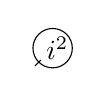
\begin{tikzpicture} \draw (0,0) circle (0.25cm) node at (0,0) {$\phantom{i}i^2$}; \draw (-.15,-.15) -- (-.225,-.225); \end{tikzpicture}}\raisebox{-3.5mm}{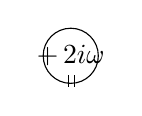
\begin{tikzpicture} \draw (0,0) circle (0.35cm) node at (0,0) {$+\,2i\omega$}; \draw (-.03,-.25) -- (-.03,-.40); \draw (.05,-.25) -- (.05,-.40); \end{tikzpicture}}
\!+ \omega^2\!
%
\edtext{%
\raisebox{-1.5mm}{\protect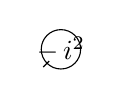
\begin{tikzpicture} \protect\draw (0,0) circle (0.25cm) node at (0,0) {$-\,i^2$}; \protect\draw (-.15,-.15) -- (-.225,-.225); \protect\end{tikzpicture}}%
$
majus
\lbrack quam\rbrack%
}{%
\lemma{\raisebox{-1.5mm}{\protect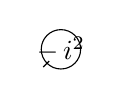
\begin{tikzpicture} \protect\draw (0,0) circle (0.25cm) node at (0,0) {$-\,i^2$}; \protect\draw (-.15,-.15) -- (-.225,-.225); \protect\end{tikzpicture}}}\Bfootnote{%
\textit{(1)}~aequ.
\textit{(2)}~majus
\textbar~quam \textit{erg. Hrsg.}~\textbar%
~\textit{L}}}
%
$%
2i^2
\raisebox{-3.5mm}{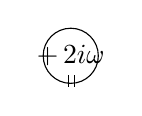
\begin{tikzpicture} \draw (0,0) circle (0.35cm) node at (0,0) {$+\,2i\omega$}; \draw (-.03,-.25) -- (-.03,-.40); \draw (.05,-.25) -- (.05,-.40); \end{tikzpicture}}.\
$
%
$\displaystyle\frac{b}{a}$
aequ.
$%
\displaystyle\frac{e^2}{i^2}.$\
%
$%
% \protect\raisebox{-1mm}{\protect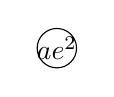
\begin{tikzpicture} \protect\draw (0,0) circle (0.25cm) node at (0,0) {$ae^2$}; \protect\end{tikzpicture}}
\ovalbox{$\displaystyle ae^2$}
+ bi^2\
\groesser\
\ovalbox{$\displaystyle ae^2$}
% \raisebox{-1.5mm}{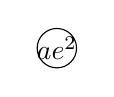
\begin{tikzpicture} \draw (0,0) circle (0.25cm) node at (0,0) {$ae^2$}; \end{tikzpicture}}
+ ai^2 + 2aei.\
$
%
$%
bi\
\groesser\
ai + 2ae.\
$
%
$%
\displaystyle\frac{b}{a}\
\groesser\
\displaystyle\frac{i + 2e}{i}.\
$
%
$%
\displaystyle\frac{e^2}{i^2}\
\groesser\
\displaystyle\frac{i + 2e}{i}.\
$
%
$%
e^2\
\groesser\
i^2 + 2ei.\
$
%
$%
\edtext{[e]}{%
\lemma{$e^2$}\Bfootnote{%
\textit{L~ändert Hrsg.}}}
\ \text{aequ.}\
i + \omega.\
$
%
Ergo
$%
\raisebox{-1.5mm}{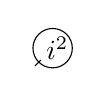
\begin{tikzpicture} \draw (0,0) circle (0.25cm) node at (0,0) {$\phantom{i}i^2$}; \draw (-.15,-.15) -- (-.225,-.225); \end{tikzpicture}}\!
+ \omega^2 +\!
\raisebox{-3.5mm}{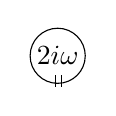
\begin{tikzpicture} \draw (0,0) circle (0.35cm) node at (0,0) {$2i\omega$}; \draw (-.03,-.25) -- (-.03,-.40); \draw (.05,-.25) -- (.05,-.40); \end{tikzpicture}}
\ \groesser\
\raisebox{-1.5mm}{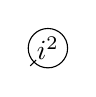
\begin{tikzpicture} \draw (0,0) circle (0.25cm) node at (0,0) {$i^2$}; \draw (-.15,-.15) -- (-.225,-.225); \end{tikzpicture}}\!
+ i^2 +\!
\raisebox{-3.5mm}{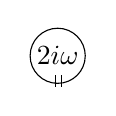
\begin{tikzpicture} \draw (0,0) circle (0.35cm) node at (0,0) {$2i\omega$}; \draw (-.03,-.25) -- (-.03,-.40); \draw (.05,-.25) -- (.05,-.40); \end{tikzpicture}}.%
$
%
Ergo
%
\edtext{$\omega^2\ \groesser \ 2i^2.$
Quod}{%
\lemma{$2i^2.$}\Bfootnote{%
\textit{(1)}~Ergo
\textit{(2)}~Quod%
~\textit{L}}}
%
possibile est.
Ideoque etiam possibile est majus esse $ae^2+bi^2$ quam $ae^2+ai^2+2aei.$
Ergo percussio%
\protect\index{Sachverzeichnis}{percussio eadem}
non potest esse semper $ae^2+bi^2$ posito distantiam
%
{\normalsize
\lbrack\textit{Text bricht ab.}\rbrack%
}
%
\pend%
\newpage%
%
\normalsize%
\pstart%
\noindent%
seu ut sit \textit{ae} aequ. \textit{bi}
seu $\displaystyle\frac{b}{a}$ aequ. $\displaystyle\frac{e}{i}.$
Ergo quaeritur
an sit $ae^2+bi^2,$
quae est vis in hoc casu concursus,%
\protect\index{Sachverzeichnis}{vis concursus}
major quam $a\,\overline{e^2 + i^2 + 2ei},$
seu an
$%
\ovalbox{$ae^2$}
% \raisebox{-2mm}{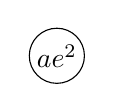
\begin{tikzpicture} \draw (0,0) circle (0.35cm) node at (0,0) {$ae^2$}; \end{tikzpicture}}
+ bi^2
\; \groesser\; 
\ovalbox{$ae^2$}
% \raisebox{-2mm}{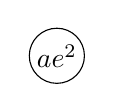
\begin{tikzpicture} \draw (0,0) circle (0.35cm) node at (0,0) {$ae^2$}; \end{tikzpicture}}
+ ai^2 + 2aei,
$
seu an
$\displaystyle\frac{b}{a}\ \groesser\ \displaystyle\frac{i + 2e}{i};$
seu quia $\displaystyle\frac{b}{a}$ aequ. $\displaystyle\frac{e}{i},$
quaestio erit%
\protect\index{Sachverzeichnis}{quaestio de percussione}
an possit esse
$\displaystyle\frac{e}{i}\ \groesser\ \displaystyle\frac{i + 2e}{i},$
seu an \textit{e} possit esse $\groesser\ i + 2e,$
\protect\rule[-2mm]{0mm}{6mm}quod est impossibile.
Ergo fieri potest
ut percussio semper sit
%
\edtext{eadem.%
\protect\index{Sachverzeichnis}{percussio eadem}
Porro hinc patet}{%
\lemma{eadem}\Bfootnote{%
\textit{(1)}~quam sic investigabimus:
\textit{(a)}~sit
\textit{(b)}~duo corpora concurrant celeritate \textit{e}~\textit{i},
\textit{(2)}~. Porro hinc patet%
~\textit{L}}}
%
vim residuam%
\protect\index{Sachverzeichnis}{vis residua}
esse illam quae
%
\edtext{est corporum,%
\protect\index{Sachverzeichnis}{vis corporum in navi}
si ambo velut in navi%
\protect\index{Sachverzeichnis}{navis}
ferantur,}{%
\lemma{est}\Bfootnote{%
\textit{(1)}~corporis. Si feratur
\textit{(2)}~corporum, si ambo
\textit{(a)}~velut quiesce\textlangle ntes\textrangle\
\textit{(b)}~velut in navi
\textit{(aa)}~in qua
\textit{(bb)}~ferantur,%
~\textit{L}}}
%
ita ut motus navis%
\protect\index{Sachverzeichnis}{motus navis}%
\protect\index{Sachverzeichnis}{navis}
sit motus centri gravitatis.%
\protect\index{Sachverzeichnis}{motus centri gravitatis}%
\protect\index{Sachverzeichnis}{centrum gravitatis}
Itaque vis residua est momentum centri gravitatis%
\protect\index{Sachverzeichnis}{momentum centri gravitatis}
seu quadratum
%
\edtext{celeritatis%
\protect\index{Sachverzeichnis}{quadratum celeritatis}
centri
\edtext{gra\textlangle vitatis\textrangle%
\protect\index{Sachverzeichnis}{centrum gravitatis}%
}{%
\lemma{gra\textlangle vitatis\textrangle}\Cfootnote{%
Wort noch lesbar im S-Film Nr.~116 der GWLB Hannover.}}
\lbrack%
\edtext{in corporum summam}{%
\lemma{in corporum summam}\Cfootnote{%
Siehe zu dieser Ergänzung \textsc{Fichant} 1994, S.~325, Anm.~1.}}%
\rbrack\
ducti.}{%
\lemma{celeritatis}\Bfootnote{%
\textit{(1)}~%
\textbar~corporum \textit{streicht Hrsg.}~%
\textbar\ ductum in v
\textit{(2)}~centri gra\textlangle vitatis\textrangle\
\textbar~in corporum summam \textit{erg.~Hrsg.}~%
\textbar\ ducti.%
~\textit{L}}}
%
\pend%
%
\pstart%
Hinc
\edtext{patet realiter
\edtext{composi\textlangle tos hos\textrangle}{%
\lemma{composi\textlangle tos hos\textrangle}\Cfootnote{%
Wörter noch lesbar im S-Film Nr.~116 der GWLB Hannover.}}
%
\lbrack89~v\textsuperscript{o}\rbrack\ %%%%    Blatt 89v
%
esse motus%
\lbrack,\rbrack}{%
\lemma{patet}\Bfootnote{%
\textit{(1)}~omnem vim
\textit{(2)}~realiter composi\textlangle tos hos\textrangle\ \lbrack89~v\textsuperscript{o}\rbrack\ esse motus%
~\textit{L}}}
%
non arbitrarie.%
\protect\index{Sachverzeichnis}{motus realiter compositi}%
\protect\index{Sachverzeichnis}{motus arbitrarie compositi}
Nimirum omnia corpora semper
velut per centrum gravitatis connexa%
\protect\index{Sachverzeichnis}{corpora per centrum gravitatis connexa}
spectari,
et ita velut unum totum aggregatum%
\protect\index{Sachverzeichnis}{aggregatum corporum}
agi ab illa causa,
quae est causa gravitatis.%
\protect\index{Sachverzeichnis}{causa gravitatis}
%%
\edlabel{LH_37_05_089v_accedendi-1}%
Est vero et alia causa in natura,%
\protect\index{Sachverzeichnis}{causa in natura}%
\protect\index{Sachverzeichnis}{natura}%
\protect\index{Sachverzeichnis}{causa percussionis}
quae
%
\edtext{efficit
ut corpora semper eadem}{%
\lemma{ut}\Bfootnote{%
\textit{(1)}~illa
\textit{(2)}~corpora semper
\textit{(a)}~eandem
\textit{(b)}~eadem%
~\textit{L}}}
%
celeritate sibi accedant%
\protect\index{Sachverzeichnis}{celeritas accessus corporum concurrentium}
vel a se invicem recedant,%
\protect\index{Sachverzeichnis}{celeritas recessus corporum concurrentium}
vel ut idem semper respectus inter corpora servetur;%
\protect\index{Sachverzeichnis}{respectus corporum concurrentium servatus}%
\edlabel{LH_37_05_089v_accedendi-2}
%%
et hae duae vires conatus habent compositos,%
\protect\index{Sachverzeichnis}{conatus compositus}
nec proinde mirum est
omnia
eo quo dixi modo,%
\protect\index{Sachverzeichnis}{modus explicandi}
ut in navi%
\protect\index{Sachverzeichnis}{navis}
posse explicari.
\pend%
%
\pstart%
Etiam idem est effectus suae causae,%
\protect\index{Sachverzeichnis}{effectus idem}
scilicet eadem distantia post ictum quae ante,%
\protect\index{Sachverzeichnis}{distantia post ictum eadem}
%
\edtext{uti eadem}{%
\lemma{uti}\Bfootnote{%
\textit{(1)}~idem
\textit{(2)}~eadem%
~\textit{L}}}
%
altitudo,%
\protect\index{Sachverzeichnis}{altitudo eadem}
seu eadem distantia a terra.%
\protect\index{Sachverzeichnis}{terra}%
\protect\index{Sachverzeichnis}{distantia a terra}
\pend%
%
\pstart%
Absolute loquendo,
seu aestimando non gravitatem%
\protect\index{Sachverzeichnis}{gravitas aestimanda}
sed appropinquationem,%
\protect\index{Sachverzeichnis}{appropinquatio aestimanda}
aestimantur vires%
\protect\index{Sachverzeichnis}{vis aestimata}%
\protect\index{Sachverzeichnis}{aestimatio virium}
seu celeritas%
\protect\index{Sachverzeichnis}{celeritas aestimata}%
\protect\index{Sachverzeichnis}{aestimatio celeritatis}
non a quadratis celeritatum in corpora ductis,%
\protect\index{Sachverzeichnis}{quadratum celeritatis ductum in corpus}
sed ab ipsis celeritatibus.%
\protect\index{Sachverzeichnis}{celeritas corporum concurrentium}
Itaque absolute quidem
in Mundo%
\protect\index{Sachverzeichnis}{mundus}
arbitror servari quantitatem motus,%
\protect\index{Sachverzeichnis}{quantitas motus in mundo servata}
etsi id non appareat in systemate.%
\protect\index{Sachverzeichnis}{systema}
Mirum quod corpora ferantur quasi in navi% ,%
\protect\index{Sachverzeichnis}{navis}
quae eorum centrum gravitatis fert;%
\protect\index{Sachverzeichnis}{centrum gravitatis corporum concurrentium}
quae vis nulla ratione perit a percussione,%
\protect\index{Sachverzeichnis}{vis a percussione perita}%
\protect\index{Sachverzeichnis}{percussio}
minuitur saltem a frictione.%
\protect\index{Sachverzeichnis}{vis a frictione minuita}%
\protect\index{Sachverzeichnis}{frictio}
\pend%
%
\pstart%
Videndum quid fieret
si quis durante percussione%
\protect\index{Sachverzeichnis}{percussio}
auferret corpora unum ab altero
ita ut ictum mox ipsa exciperent,%
\protect\index{Sachverzeichnis}{ictus exceptus}
tunc pereunte ictu%
\protect\index{Sachverzeichnis}{ictus periens}
et in ventos evanescente,%
\protect\index{Sachverzeichnis}{ictus evanescens}%
\protect\index{Sachverzeichnis}{ventus}
ambo corpora pergerent%
\protect\index{Sachverzeichnis}{corpus pergens}
celeritate centri gravitatis.%
\protect\index{Sachverzeichnis}{celeritas centri gravitatis}%
\protect\index{Sachverzeichnis}{centrum gravitatis corporum concurrentium}
\pend%
\newpage
\pstart%
Sint corpora%
\protect\index{Sachverzeichnis}{corpora concurrentia}
%
\edtext{concurrentia duo}{%
\lemma{concurrentia}\Bfootnote{\hspace{-0,5mm}%
\textbar~quaecunque \textit{gestr.}~%
\textbar\ duo%
~\textit{L}}}
%
\textit{a}~\textit{b},
quorum celeritates \textit{e}~\textit{i}%
\protect\index{Sachverzeichnis}{celeritas corporum concurrentium}
ante concursum,%
\protect\index{Sachverzeichnis}{celeritas ante concursum}
et $\epsilon$~\textit{y} post concursum,%
\protect\index{Sachverzeichnis}{celeritas post concursum}%
\protect\index{Sachverzeichnis}{concursus corporum}
\protect\rule[-4mm]{0mm}{10mm}erit via centri gravitatis:%
\protect\index{Sachverzeichnis}{via centri gravitatis}%
\protect\index{Sachverzeichnis}{centrum gravitatis corporum concurrentium}
%
\edtext{}{%
{\xxref{LH_35_07_089v_tflk-1}{LH_35_07_089v_tflk-2}}%
{\lemma{est \lbrack...\rbrack\ partes}\Cfootnote{%
%
Vielmehr gilt, dass die Differenz der Geschwindigkeiten vor dem Stoß (\textit{e}, \textit{i}) den Fall der \textit{assecutio}, die Summe derselben Geschwindigkeiten den des \textit{occursus} ausdrückt.
Vgl. N.~\ref{dcc_08}, S.~\refpassage{LH_37_05_087v_eskfz-1}{LH_37_05_087v_eskfz-2}.
Leibniz selbst bemerkt einige Zeilen weiter unten (S.~\refpassage{LH_35_07_089v_kruwk-1}{LH_35_07_089v_kruwk-2}), dass die auf diesen Setzungen beruhende Rechnung nicht stimmig sei.
Siehe hierüber auch \textsc{Fichant} 1994, S.~327\,f.\cite{01056}%
}}}%
%
\edtext{$\displaystyle\frac{ae\,\leibvdash\, bi}{a+b},$
\edlabel{LH_35_07_089v_tflk-1}%
est autem}{%
\lemma{$\displaystyle\protect\frac{ae\,\leibvdash\, bi}{a+b},$}\Bfootnote{%
\textit{(1)}~quae ducta in summam corporum dabit vim qua corpora nitentur progredi via centri,
\textit{(2)}~nempe $ae\pleibvdash bi$
\textit{(3)}~est autem%
~\textit{L}}}
%
$\leibvdash$ aequ. $-$
quando corpora sibi occurrunt,%
\protect\index{Sachverzeichnis}{corpora sibi occurrentia}
et $\leibvdash$ aequ. $+$
quando tendunt in easdem partes.%
\protect\index{Sachverzeichnis}{corpora in easdem partes tendentia}%
\edlabel{LH_35_07_089v_tflk-2}
Haec quantitas
%
\edtext{quadrata%
\protect\index{Sachverzeichnis}{quantitas quadrata}
et in summam corporum ducta,%
\protect\index{Sachverzeichnis}{summa corporum concurrentium}
dabit:}{%
\lemma{quadrata}\Bfootnote{%
\textit{(1)}~dabit:
\textit{(2)}~et in % summam corporum 
\lbrack...\rbrack\ ducta, dabit:%
~\textit{L}}}
%
$\displaystyle\frac{a^2e^2+b^2i^2\,\leibvdash\,2abei}{a+b}$
\protect\rule[-4mm]{0mm}{10mm}quae est
%
\edtext{vis qua}{%
\lemma{vis}\Bfootnote{\hspace{-0,5mm}%
\textbar~residua \textit{gestr.}
\textbar\ qua summa%
~\textit{L}}}
%
summa corporum pergere conatur,%
\protect\index{Sachverzeichnis}{vis summae corporum}
quae subtracta a $ae^2+bi^2$
relinquet vim percussionis;%
\protect\index{Sachverzeichnis}{vis percussionis}
fiet ergo:
\newline%
$\displaystyle\frac{%
\raisebox{-2.5mm}{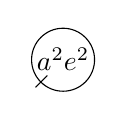
\begin{tikzpicture} \draw (0,0) circle (0.4cm) node at (0,0) {$a^2e^2$}; \draw (-.2,-.2) -- (-.35,-.35); \end{tikzpicture}}+abi^2+abe^2\raisebox{-2.5mm}{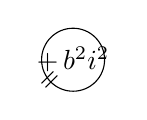
\begin{tikzpicture} \draw (0,0) circle (0.4cm) node at (0,0) {$+\,b^2i^2$}; \draw (-.25,-.15) -- (-.4,-.3); \draw (-.2,-.2) -- (-.35,-.35); \end{tikzpicture}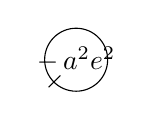
\begin{tikzpicture} \draw (0,0) circle (0.4cm) node at (0,0) {$-\,a^2e^2$}; \draw (-.2,-.2) -- (-.35,-.35); \end{tikzpicture}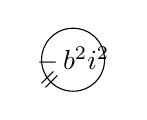
\begin{tikzpicture} \draw (0,0) circle (0.4cm) node at (0,0) {$-\,b^2i^2$}; \draw (-.25,-.15) -- (-.4,-.3); \draw (-.2,-.2) -- (-.35,-.35); \end{tikzpicture}}\,\leibvdash\, 2abei%
}{a+b}$
%
seu
%
\edtext{%
$\displaystyle\frac{ab}{a+b}\;\protect\overline{\protect\framebox{2}\:\pmA\,e\, \pmB\, i},$%
}{%
\lemma{\textit{Am Rand:}}\Afootnote{%
Si \textit{i} aequ. 0,
oritur percussio%
\protect\index{Sachverzeichnis}{percussio}
quam alibi\textsuperscript{\lbrack a\rbrack}
esse dixi
cum corpus impingit%
\protect\index{Sachverzeichnis}{corpus impingens}
in quiescens.%
\protect\index{Sachverzeichnis}{corpus quiescens}
\newline\vspace{-0.3em}%
\newline%
{\footnotesize%
\textsuperscript{\lbrack a\rbrack}~alibi:
N.~\ref{dcc_06-1}, %??S01\textsubscript{7}, 
S.~\refpassage{LH_35_09_23_014r_percussioinquiescens}{LH_35_09_23_014r_percussioinquiescens}\,ff.
Siehe hierzu \textsc{Fichant} 1994, S.~163 u.~328, Anm.~1.\cite{01056}%
}}}
%
\protect\rule[-2mm]{0mm}{9mm}quam vim patet
perfectissimam habere relationem similem%
\protect\index{Sachverzeichnis}{relatio similis}
ad duo corpora,%
\protect\index{Sachverzeichnis}{corpora concurrentia}
%
\edtext{est scilicet
$\displaystyle\frac{ab}{a+b}$
ductum in quadratum distantiae corporum.%
\protect\index{Sachverzeichnis}{quadratum distantiae}%
\protect\index{Sachverzeichnis}{distantia corporum concurrentium}%
}{%
\lemma{scilicet}\Bfootnote{%
\textit{(1)}~factum
\textit{(2)}~quadratum corporum
\textit{(3)}~$\displaystyle\protect\frac{ab}{a+b}$ ductum % in quadratum 
\lbrack...\rbrack\ distantiae corporum.%
~\textit{L}}}
%
\pend%
%
\pstart%
Corporum distantia%
\protect\index{Sachverzeichnis}{corpora concurrentia}%
\protect\index{Sachverzeichnis}{distantia corporum concurrentium}
est $e \:\pleibdashv\: i,$
et quando intelliguntur eam conficere
%
\edtext{celeritate corporibus reciproca,%
\protect\index{Sachverzeichnis}{celeritas corporibus reciproca}%
}{%
\lemma{celeritate}\Bfootnote{%
\textit{(1)}~distantiis reciproca,
\textit{(2)}~corporibus reciproca,%
~\textit{L}}}
%
tunc unius
%
\edtext{celeritas,%
\protect\index{Sachverzeichnis}{celeritas corporum concurrentium}
scil. ipsius \textit{a},
erit}{%
\lemma{celeritas}\Bfootnote{%
\textit{(1)}~\textbar~erit \textit{streicht Hrsg.}~\textbar\
\textit{(2)}~, scil. ipsius \textit{a} erit.%
~\textit{L}}}
%
$\displaystyle\frac{b}{a+b}\,%
\overline{e\,\leibdashv\,i},$
et alterius,%
\protect\index{Sachverzeichnis}{celeritas corporum concurrentium}
\textit{b}, \makebox[1.0\textwidth][s]{celeritas erit
$\displaystyle\frac{a}{a+b}\,%
\overline{e\,\leibdashv\,i},$
adeoque\protect\rule[-4mm]{0mm}{10mm} vis illius erit:%
\protect\index{Sachverzeichnis}{vis corporum concurrentium}
$\displaystyle\frac{b^2a}{a^2+2ab+b^2}\,%
\overline{e^2\,\leibdashv\,2ei+i^2},$
vis alterius%
\protect\index{Sachverzeichnis}{vis corporum concurrentium}}
\pend
\newpage
\pstart
\noindent
$\displaystyle\frac{a^2b}{a^2+2ab+b^2}\,%
\overline{e^2\,\leibdashv\,2ei+i^2},$
addantur simul fiet:
$\displaystyle\frac{b^2a+a^2b}{a^2+2ab+b^2}\,%
\overline{e^2\,\leibdashv\,2ei+i^2},$
seu dividendo fractionis \protect\rule[-4mm]{0mm}{10mm}nominatorem%
\protect\index{Sachverzeichnis}{fractio}%
\protect\index{Sachverzeichnis}{nominator fractionis}
pariter ac numeratorem%
\protect\index{Sachverzeichnis}{numerator fractionis}
per $a+b,$
fiet
$\displaystyle\frac{ab}{a + b}\,%
\overline{e^2\,\leibdashv\,2ei+i^2}.$
\edlabel{LH_35_07_089v_kruwk-1}%
Qui calculus differre videtur \protect\rule[-4mm]{0mm}{10mm}a superiore,%
\protect\index{Sachverzeichnis}{calculus}
nam paulo ante fiebat
$\displaystyle\frac{ab}{a+b}\,%
\overline{e^2\,\leibvdash\,2ei+i^2}.$
Sed posterior est verior,%
\protect\index{Sachverzeichnis}{calculus}
neque enim
proprie loquendo
subtrahendae a se invicem%
\protect\index{Sachverzeichnis}{vires a se invicem subtrahendae}
%
\edtext{hae vires duplices.%
\edlabel{LH_35_07_089v_kruwk-2}%
}{%
\lemma{hae}\Bfootnote{%
\textit{(1)}~duae
\textit{(2)}~vires duplices.%
~\textit{L}}}
%
\pend%
%
\pstart%
Conatus naturae unus est,%
\protect\index{Sachverzeichnis}{conatus naturae}
efficiendi
ut centrum gravitatis eadem procedat via,%
\protect\index{Sachverzeichnis}{centrum gravitatis}%
\protect\index{Sachverzeichnis}{via centri gravitatis eadem}
et aeque alte%
\protect\index{Sachverzeichnis}{ascensus centri gravitatis}
%
\edtext{assurgere possit ante}{%
\lemma{assurgere}\Bfootnote{%
\textit{(1)}~ante
\textit{(2)}~possit ante%
~\textit{L}}}
%
ictum quam post ictum.%
\protect\index{Sachverzeichnis}{ictus}
Alter naturae conatus est,%
\protect\index{Sachverzeichnis}{conatus naturae}
ut corpora ipsa%
\protect\index{Sachverzeichnis}{corpora concurrentia}
aeque a se invicem recedere possint%
\protect\index{Sachverzeichnis}{recessus corporum concurrentium}%
\protect\index{Sachverzeichnis}{corpora a se invicem recedentia}
ante ictum et post ictum;%
\protect\index{Sachverzeichnis}{ictus}
seu ut eandem semper vim in se invicem,
seu percutiendi,%
\protect\index{Sachverzeichnis}{vis percutiendi}
habere possint.%
\protect\index{Sachverzeichnis}{percussio eadem}
Quemadmodum ex priori eandem semper vim retinent%
\protect\index{Sachverzeichnis}{vis retenta}
percutiendi tellurem,%
\protect\index{Sachverzeichnis}{tellus}%
\protect\index{Sachverzeichnis}{vis percutiendi tellurem}
etiam ut singulare corpus spectatam.%
\protect\index{Sachverzeichnis}{corpus singulare}
\pend%
%\vspace{1.0em}%
%%
%\pstart%
%\noindent%
%\lbrack\textit{Am Rand, schräg:}\rbrack\
%\pend%
%\vspace{0.5em}%
%
\pstart%
%\noindent%
Conclusimus inquisitionem de regulis motus,%
\protect\index{Sachverzeichnis}{inquisitio de regulis motus}%
\protect\index{Sachverzeichnis}{regula motus}
et satisfecimus tandem nobis.
\pend%
\vspace{1.0em}%
%
\pstart%
\noindent%
\lbrack\textit{Am Rand, auf den Abschnitt S.~\refpassage{LH_35_07_089v_kruwk-1}{LH_35_07_089v_kruwk-2} bezogen:}\rbrack\
\pend%
\vspace{0.5em}%
%
\pstart%
\noindent%
Imo error est nullus.%
\protect\index{Sachverzeichnis}{error nullus}
Nam si a vi tota%
\protect\index{Sachverzeichnis}{vis corporum concurrentium tota}
%
$ae^2 + bi^2$
%
%\edtext{}{%
%\lemma{\textit{Am Rand:}}\Afootnote{%
%$by\,(\leibvdash)\,a\epsilon$ aequ. $ae\,\leibvdash\,bi$\\
%$(\leibdashv)\,\epsilon+y$ aequ. $e\,\leibdashv\,i$\\
%multiplicetur posterior aequatio per $-b$ et addatur productum priori,
%fiet:
%$(\leibvdash)\protect\underset{\displaystyle b}{a}\epsilon$ aequ. $\protect\underset{\displaystyle -b}{+a}e\,\leibvdash\,2bi,$
%seu $\epsilon$ aequ. $\displaystyle\protect\frac{\protect\underset{\displaystyle -b}{+a}e\,\leibvdash\,2bi}{(\leibvdash)\overline{a+b}}.$
%Aliter:
%multiplicetur posterior aequatio per $+a$ et addatur priori,
%fiet:
%$\protect\underset{\displaystyle +b}{+a}y$ aequ. $2ae\,\protect\underset{\displaystyle \leibvdash\,b}{\leibdashv a}i,$
%seu \textit{y} aequ. $\displaystyle\protect\frac{2ae\protect\underset{\displaystyle \leibvdash\,a}{\leibdashv b}i}{a+b}.$}}
%
auferatur vis percussionis%
\protect\index{Sachverzeichnis}{vis percussionis}
$\displaystyle\frac{ab}{a + b}\:%
\overline{e^2\,\leibdashv\,2ei + i^2}$
fiet:
%
$\displaystyle\frac{a^2e^2
\raisebox{-2.5mm}{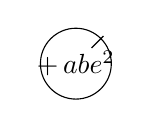
\begin{tikzpicture} \draw (0,0) circle (0.45cm) node at (0,0) {$+\,abe^2$}; \draw (.2,.2) -- (.35,.35); \end{tikzpicture}}
\raisebox{-2.5mm}{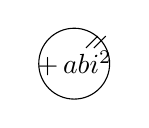
\begin{tikzpicture} \draw (0,0) circle (0.45cm) node at (0,0) {$+\,abi^2$}; \draw (.15,.2) -- (.3,.35); \draw (.25,.2) -- (.4,.35); \end{tikzpicture}}
+b^2i^2\raisebox{-2.5mm}{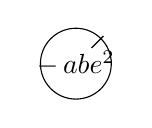
\begin{tikzpicture} \draw (0,0) circle (0.45cm) node at (0,0) {$-\,abe^2$}; \draw (.2,.2) -- (.35,.35); \end{tikzpicture}}\,
\leibvdash\,2abei\,
\raisebox{-2.5mm}{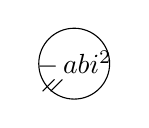
\begin{tikzpicture} \draw (0,0) circle (0.45cm) node at (0,0) {$-\,abi^2$}; \draw (-.15,-.2) -- (-.3,-.35); \draw (-.25,-.2) -- (-.4,-.35); \end{tikzpicture}}%
}{a+b}$
%
aequ.
$\displaystyle\frac{\overline{ae\,\leibvdash\,bi}\:\framebox{2}}{a+b},$%
\rule[-4mm]{0mm}{0mm}
%
\edtext{seu via centri}{%
\lemma{seu}\Bfootnote{%
\textit{(1)}~vis
\textit{(2)}~via%
~\textit{L}}}
%
gravitatis in summam corporum ducta,%
\protect\index{Sachverzeichnis}{centrum gravitatis}%
\protect\index{Sachverzeichnis}{summa corporum}%
\protect\index{Sachverzeichnis}{via centri gravitatis in summam corporum ducta}
seu vis quam corpora habent pergendi.%
\protect\index{Sachverzeichnis}{vis pergendi corporum concurrentium}
\pend%
\vspace{1.0em}%
%
\pstart%
\noindent%
\lbrack\textit{Nachträglich hinzugefügt:}\rbrack\
\pend%
\vspace{0.5em}%
%
\pstart%
\noindent%
$by\,(\pleibvdash\!)\,a\epsilon$ aequ. $ae\,\leibvdash\,bi.$
\quad%
$(\pleibdashv\!)\,\epsilon + y$ aequ. $e\,\pleibdashv\,i.$
%
\newline%
Multiplicetur posterior aequatio per $-\:b$%
\protect\index{Sachverzeichnis}{aequatio}
et addatur productum priori,%
\protect\index{Sachverzeichnis}{productum}
\newline%
fiet:
$(\pleibvdash\!)\protect\underset{\displaystyle b}{a}\; \epsilon$
aequ.\protect\rule[-4mm]{0mm}{10mm}
$\protect\underset{\displaystyle -b}{+a}e\,\pleibvdash\,2bi,$
seu
$\epsilon$
aequ.
$\displaystyle\protect\frac{\protect\underset{\displaystyle -b}{+a}\; e\,\leibvdash\,2bi}{(\leibvdash)\overline{a+b}}.$
\newline%
Aliter:\protect\rule[-2mm]{0mm}{7mm}
multiplicetur posterior aequatio per $+\:a$%
\protect\index{Sachverzeichnis}{aequatio}
et addatur priori,
\newline%
fiet:
$\protect\underset{\displaystyle +b}{+a}\; y$
aequ.
$2ae\,\protect\underset{\displaystyle \leibvdash\,b}{\leibdashv a}i,$
seu
\textit{y} aequ.
$\displaystyle\protect\frac{2ae\; \protect\underset{\displaystyle \leibvdash\,a}{\leibdashv b}i}{a+b}.$
\pend%
%
\count\Bfootins=1200%
\count\Afootins=1200%
\count\Cfootins=1200
%\pstart
%\normalsize
%Scheda decima.
%\pend
%
%
%%%%    Ende des Textes auf Blatt 89v